\documentclass[10pt,conference,compsocconf]{IEEEtran}

\usepackage{hyperref}
\usepackage{graphicx}
\usepackage{xcolor}
\usepackage{blindtext, amsmath, comment, subfig, epsfig }
\usepackage{grffile}
\usepackage{caption}
%\usepackage{subcaption}
\usepackage[utf8]{inputenc}


\title{CS-523 SecretStroll Report}
\author{Laval Maxime, Carles Victor}
\date{April 2020}

\begin{document}

\maketitle

\section{Attribute-based credential}

\subsection{Issuance Protocol}

The first step of the Attribute based credential authentication is the issuance of the credentials. To do so, we decided that the user's attributes would be his username, whereas the issuer's attributes would be all the subscriptions the user sends to it. This way, we have the union of both subsets as the whole set of all the user's attributes. As a specification of implementation, we decided to create dictionaries for the user and issuer attributes that map $Y_{i}$ to the corresponding $a_{i}$. All $Y_{i}$ are computed by the server when generating the keys, and they are stored in the public key at the index corresponding to each attribute, the last one being the username. We also stored all the attributes in the public key, as it is easier for some methods to access attribute and retrieve indexes based on the size. 
This way, if a method needs the $Y_{i}$ of a given attribute, it can simply search for the index i of the attribute in the pk and get the value at index i+1 (since g is the first value stored in the pk).
When creating the issue request, the user sends a commitment C to the issuer, as well as a challenge c (which is a sha256 hash $H(pk,C,R)$), and a pre-computed response s. Since it is the user that computes the response, the proof is non-interactive, meaning that the issuer doesn't have to do anything except verifying that the challenge he receives was correctly computed, hence proving that the user really has the attributes. Since the issuer doesn't have the user's attributes, it can't compute $C = g^t \prod_{i e U}{Y_{i}^{a_{i}}}$ . 
But, it can compute R'. 
\\	
\hspace{1cm}
R is computed by the user as $g^{rt} \prod_{i e U}{Y_{i}^{ra_{i}}}$, where $rt$ and $ra_{i}$, for i e U, are random values chosen by the user. 
\\	
\hspace{1cm}

$ R' = C^c g^{st} \prod_{i e U}{Y_{i}^{sa_{i}}}$, where $st = rt - c*t$ and $sai = ra_{i} - c*a_{i}$ for i e U. This way, this should all simplify in a way that R' is equal to R, resulting in a same hash a c. The issuer doesn't have to know the user's attributes, it just has to know the indexes to find the corresponding $Y_{i}$ for the responses values $sai$.
If R = R', then the proof is valid, and the user can obtain his credentials. The credentials are all his subscriptions and his username.

\subsection{Showing Protocol}
To prove that the user has the right credentials, we use a similar method as the previous zero-knowledge proof. The user this time sends $C = e(sigma_{1}',g^{tilda})^t \prod_{i e H} e(sigma_{1}',Y_{i}^{tilda})^{a_{i}}$ and computes $ R = e(sigma_{1}',g^{tilda})^{rt} \prod_{i e H} e(sigma_{1}',Y_{i}^{tilda})^{ra_{i}}$ 
\\	
\hspace{1cm}

Whereas the server computes \\ $ R = C^c  e(sigma_{1}',g^{tilda})^{st} \prod_{i e H} e(sigma_{1}',Y_{i}^{tilda})^{sa_{i}}$. Once again, the obtained value hashed together with C and pk should be equal to the challenge c. If this is the case, than the user has correctly proved that he has the credentials, without having to show them to the server. 


\subsection{Test}d
How did you test the system?
You need to test the correct path and at least two failure paths.

\subsection{Evaluation}
Evaluate your ABC: report communication and computation stats (mean and standard
deviation). Report statistic on key generation, issuance, signing, and
verification.

\section{(De)Anonymization of User Trajectories}

\subsection{Privacy Evaluation} 
	To conduct a privacy analysis, we first have to define the adversarial model. One such adversary could be an eavesdropper sniffing the network to access all queries and POIs, supposing everything is sent in clear, or someome having access to the dataset if it is stored in the app. From this set of queries and POIs, the adversary would be able to infer many things for a given IP address. First of all, the adversary can group the POIs by type. For instance, POIs such as villa or appartment block would correspond to places in which people reside. If the adversary makes an exhaustive search and check that, for some queries of the user, a POI of this type frequently occurs, and that its location is always unique, he can easily deduce that this corresponds to the user's home. Same goes for the place of work. By doing that, it is easy for the adversary to determine where a target lives, where he works, or simply the places he goes to the most, whenever the user uses the app at those locations. He could then be able to associate an IP address to the user's identity.
\\	
\hspace{1cm}
\\
	We can group other kind of informations, such as habits. This could be particularly useful if the app wanted to collect data and use them for ad-targeting for instance. All we have to do is group all hobbies-like POIs (club, bar, gym, dojo etc), and count the number of queries with locations corresponding to those types. In the part2.ipynb file, we have computed all such activities for a target IP and grouped them into the following graph. As we can see, the target likes clubbing a lot, and going to bars sometimes. We can even get the exact location of clubs and bars in question.
Same goes for places to eat. The adversary can also determine the time the user spends at a given place with the timestamps. 
	
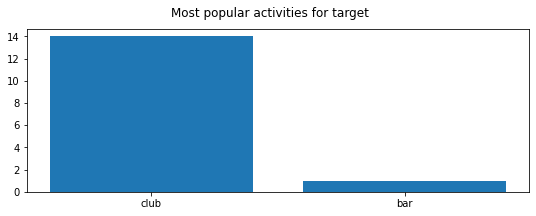
\includegraphics[scale=0.45]{target_activities}
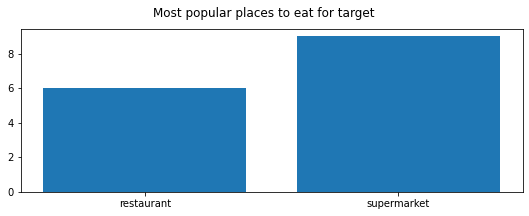
\includegraphics[scale=0.45]{target_places_to_eat}
	 
	Although we haven't computed it for this evaluation, we could think of a lot of other types of attacks, such as grouping different users by types of POIs to collect even more data and identify common habits between users.
	 
\subsection{Defenses}

	The main privacy risk with this app results from the fact that the user's locations are way too precise. We could add noise to the result in a way to obfuscate the real user's location, but there is an even simpler method. As we know, all POIs are distributed into cells. What we can do is, instead of using the user's real location to get the nearby POIs, we return all POIs in the same cell as the user. This way, the only thing an adversary could know from a user would be the cell he was in at the time of the query, which doesn't give much information on whether he was at home, at work, in a bar etc.
Since we converted the latitude longitude attributes to the cell id using the location to cell id method, there are no more unique locations, making it impossible for the adversary to determine the user's exact location (let's remind us that the grid cell is the size of a few kilometers square). Hence, the privacy of the user's location is respected. The trade-off is relatively small, as user will still be able to get the POIs he's interested in near his location, although some will be more far.
As we can see in the following graph, if the adversary tries to determine where the user spends most of his time, it is hard to tell.

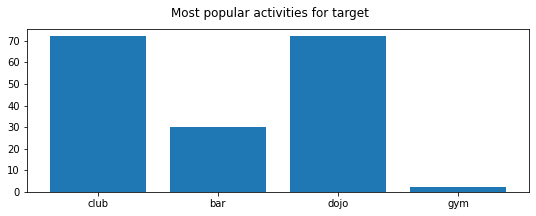
\includegraphics[scale=0.5]{target_activities_defense}

The problem is that it doesn't increase drastically the privacy, as for instance a cell containing only one type of POI could still let the adversary infer some information on the user's habit. 
What we could do is add dummy values to the POIs, although this would greatly reduce the utility of the app. We could also add noise to the timestamp so that an adversary can't determine the exact time the user was at some place.
	 
\section{Cell Fingerprinting via Network Traffic Analysis}

\subsection{Implementation details}
Provide a description of your implementation here. You should provide details on your data collection methods, feature extraction, and classifier training.

\subsection{Evaluation}
Provide an evaluation of your classifier here -- the metrics after 10-fold cross validation.

\subsection{Discussion and Countermeasures}
Comment on your findings here. How well did your classifier perform? What factors could influence its performance? Are there countermeasures against this kind of attack?

\bibliographystyle{IEEEtran}
\bibliography{bib}
\end{document}
